\section{Architettura}

\subsection{Introduzione}
\par Il prodotto ChatSQL è basato su un'architettura client-server. Il client è l'interfaccia attraverso la quale gli utenti interagiscono con il sistema, come ad esempio un browser web. In altre parole, il client è il componente che richiede risorse o servizi. Il server è l'applicazione che riceve ed elabora le richieste provenienti da uno o più client, fornendo risposte appropriate.

\begin{figure}[H]
  \centering
  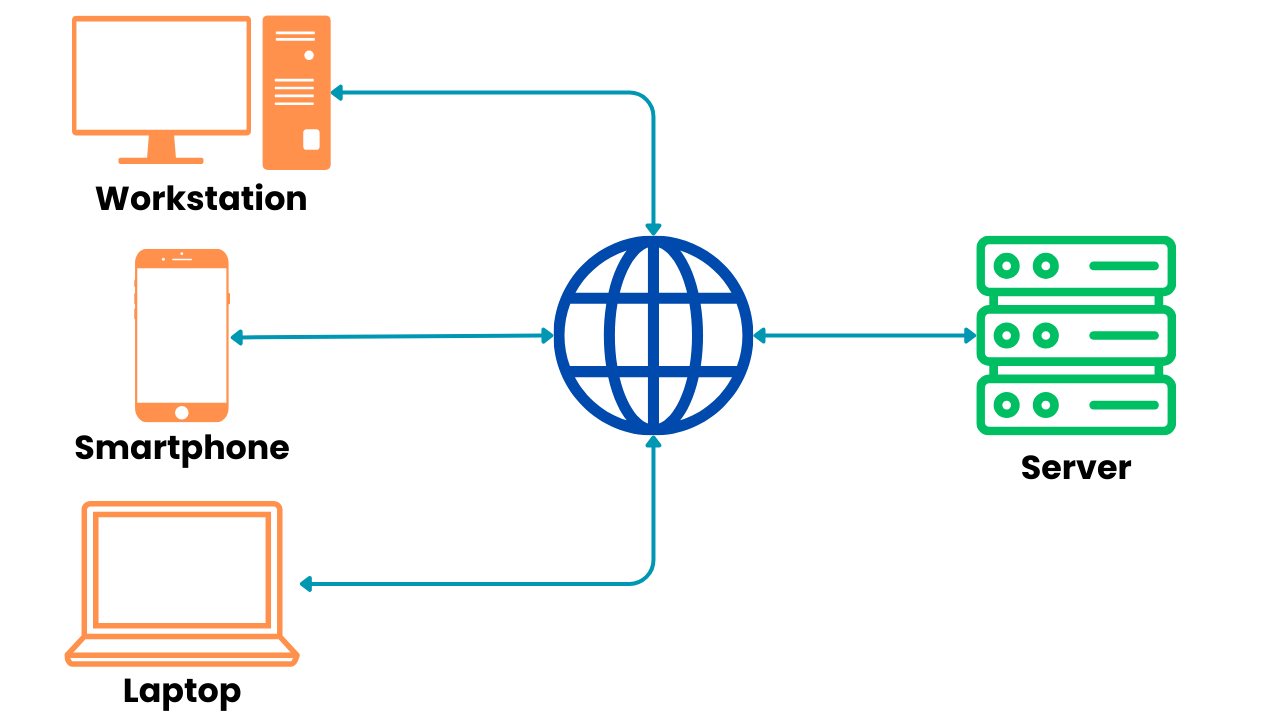
\includegraphics[width=0.95\textwidth]{assets/client_server.png}
  \caption{Architettura client-server}
\end{figure}

\par Per migliorare lo sviluppo collaborativo, la modularità e la manutenibilità, il sistema è stato suddiviso in due componenti principali:
\begin{itemize}
<<<<<<< HEAD
  \item \textbf{Front-end}: è la porzione di un sistema che l'utente visualizza e con cui può interagire. Il front-end è sviluppato utilizzando il framework \glossario{Vue.js} ed è responsabile dell'interfaccia grafica, che deve essere intuitiva, funzionale e accattivante. Trasmette le richieste dell'utente al back-end e visualizza i risultati ottenuti;
  \item \textbf{Back-end}: è il segmento che gestisce la logica di business, l'elaborazione dei dati e la comunicazione con i database e altri servizi. Il back-end è sviluppato utilizzando il framework \glossario{FastAPI}.
=======
  \item \textbf{Front-end}: la porzione di un sistema che l'utente visualizza e con cui può interagire. Il front-end è sviluppato utilizzando il framework \glossario{Vue.js} ed è responsabile dell'interfaccia grafica, che deve essere intuitiva, funzionale e accattivante. Trasmette le richieste dell'utente al back-end e visualizza i risultati ottenuti;
  \item \textbf{Back-end}: il segmento che gestisce la logica di business, l'elaborazione dei dati e la comunicazione con i database e altri servizi. Il back-end è sviluppato utilizzando il framework \glossario{FastAPI}.
>>>>>>> main
\end{itemize}

\vspace{0.5\baselineskip}
\par La comunicazione tra il front-end e il back-end avviene tramite chiamate \glossario{API}. Il team segue le linee guida e i principi definiti da REST (representational state transfer), uno stile architetturale che impone condizioni sul funzionamento di un'API. Le REST API (o RESTful API) sono stateless, il che significa che ogni richiesta HTTP deve includere tutte le informazioni necessarie per elaborarla. Questo riduce il carico sul server e migliora la scalabilità. Inoltre, l’approccio stateless agevola l'implementazione di sistemi di caching, migliorando le prestazioni complessive. Una REST API è simile a un sito web in esecuzione in un browser con funzionalità HTTP integrata. Le operazioni sono basate su metodi HTTP standard come GET, POST, PUT e DELETE.

\vspace{0.5\baselineskip}
\par La persistenza delle informazioni dei dizionari (nome, descrizione, ecc.) è garantita dalla presenza di un database, che memorizza anche gli operatori registrati nel sistema. Il database è implementato utilizzando SQLite. Di seguito è riportata l'architettura ad alto livello della web app.

\begin{figure}[H]
  \centering
  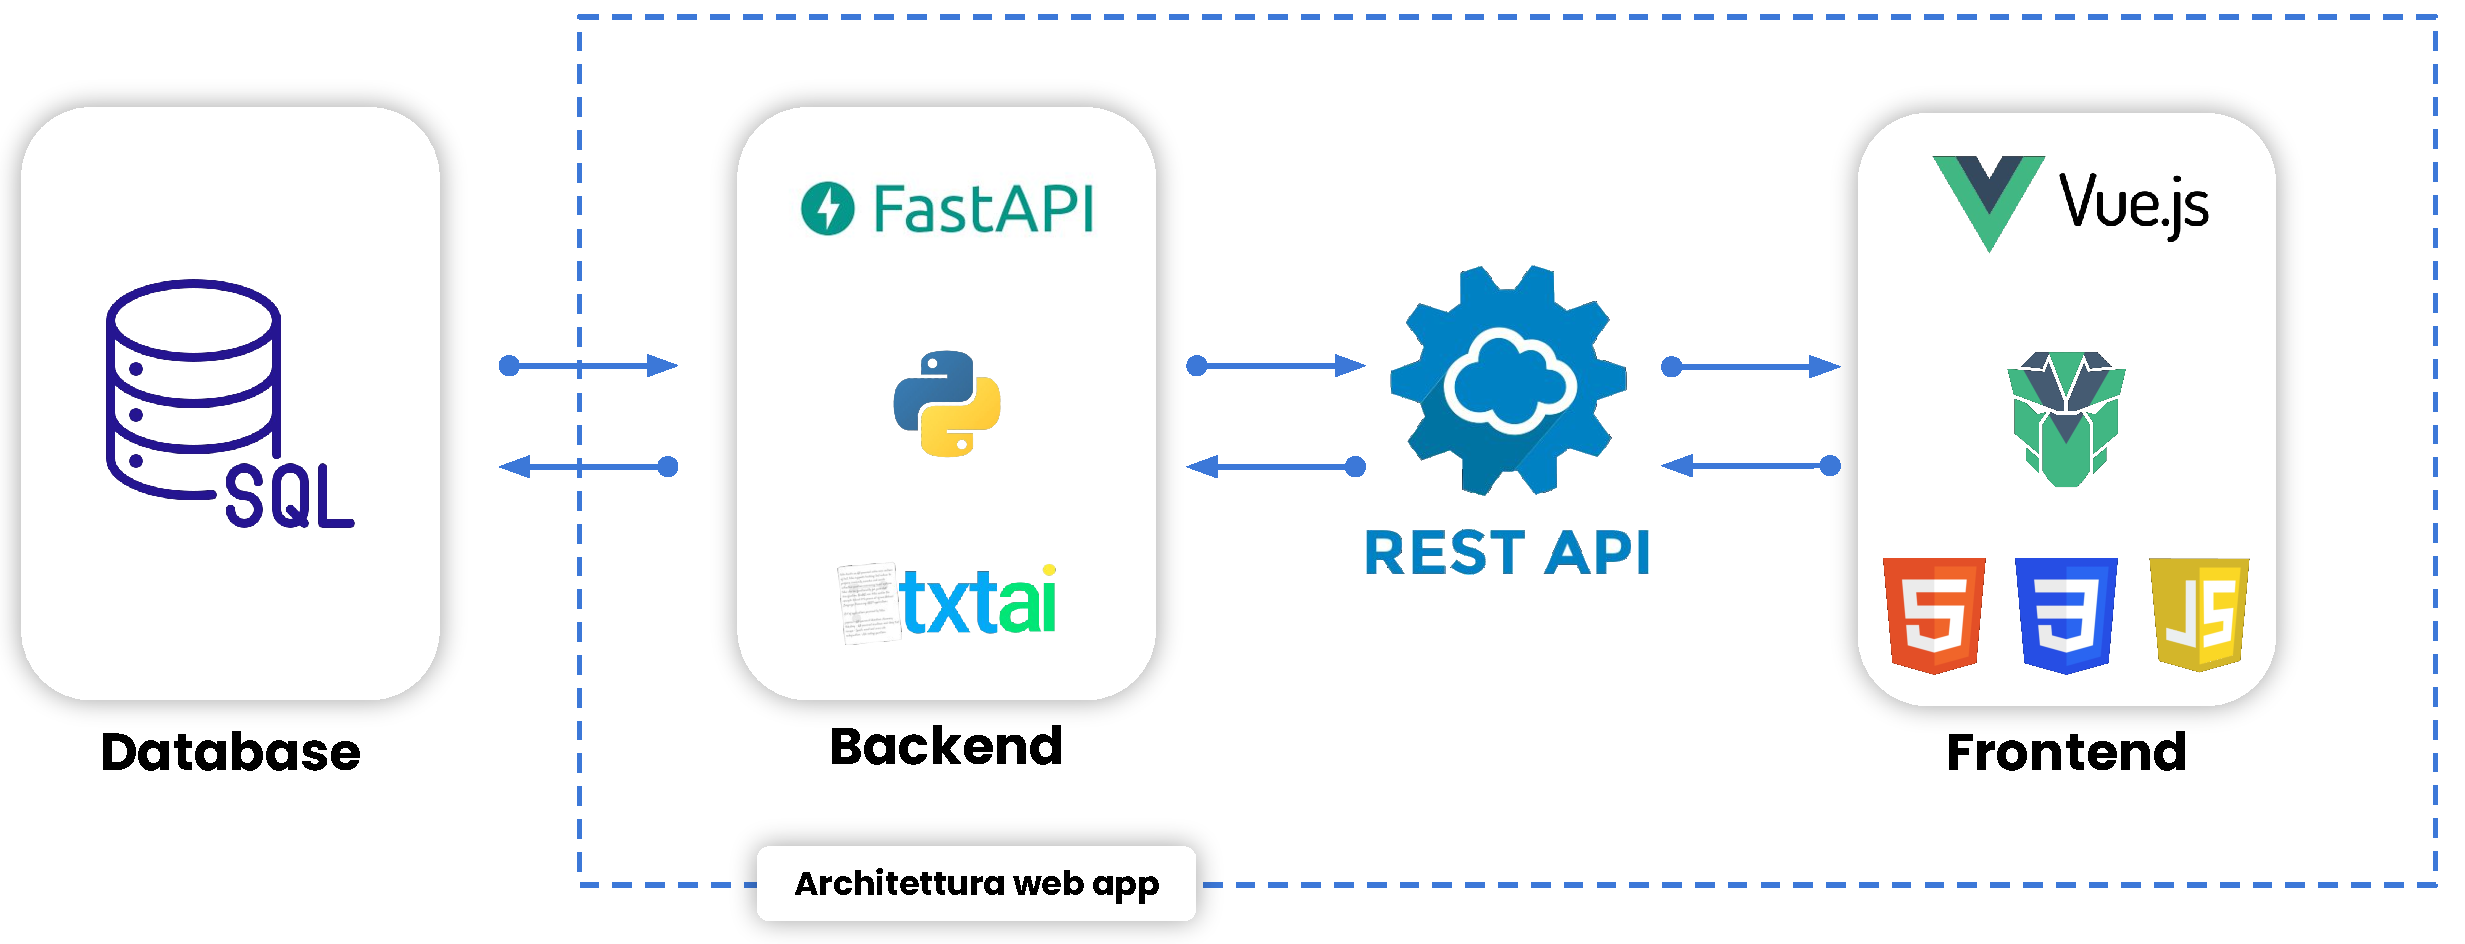
\includegraphics[width=\textwidth]{assets/architettura_web_app.pdf}
  \caption{Architettura web app}
\end{figure}

\subsection{Assemblaggio dei componenti}
\par Docker Compose viene utilizzato per gestire applicazioni multi-container, permettendo di assemblare diversi servizi che compongono un'applicazione. Nel contesto di ChatSQL, il team ha creato i seguenti container Docker:
\begin{itemize}
  \item \textbf{backend}: espone l'interfaccia di backend sulla porta 8000. All'indirizzo \textit{localhost:8000/docs} è possibile consultare la documentazione interattiva delle API. Inoltre, sono disponibili dettagli sui Data Transfer Objects (DTO);
  \item \textbf{frontend}: espone l'interfaccia utente sulla porta 5173.
\end{itemize}

\subsection{Struttura del sistema}

\subsubsection{Back-end}

\par La struttura organizzativa del back-end segue i principi dello stile architetturale scelto, al fine di semplificare il processo di traduzione della progettazione in codice. Il back-end è suddiviso nelle seguenti cartelle:

\begin{minipage}{\textwidth}
  \dirtree{%
    .1 backend.
    .2 TODO.
    .2 TODO.
  }
\end{minipage}
\subsubsection{Back-end}

\par La struttura organizzativa del back-end segue i principi dello stile architetturale scelto, al fine di semplificare il processo di traduzione della progettazione in codice. Il back-end è suddiviso nelle seguenti cartelle:

\begin{minipage}{\textwidth}
  \dirtree{%
    .1 backend.
    .2 TODO.
    .2 TODO.
  }
\end{minipage}